\documentclass[11pt]{article}
\usepackage[pdftex]{graphicx}
\usepackage{amsmath, amsthm, amssymb, amsfonts, mathtools, graphicx, enumerate}
\usepackage{times}
\usepackage{booktabs}
\usepackage{url}
\usepackage{color,soul}
\usepackage{enumerate}
\usepackage{listings}
%%\usepackage{enumitem}
\newcommand{\R}{\mathbb{R}}
\setlength{\parindent}{0pt}
\setlength{\parskip}{1ex}
\setlength{\oddsidemargin}{0.0in}
\setlength{\textwidth}{6.5in}
\setlength{\topmargin}{-0.5in}
\setlength{\textheight}{9.0in}
\newcommand{\RR}{\mathbb{R}}
\newcommand{\labelsymbol}{t}
\newcommand{\answer}[1]{{\mbox{}\color{red}{#1}}}
\newcommand{\emptycheck}{\text{(\hspace{-.75ex}(\hspace{3ex})\hspace{-.75ex})}}
\newcommand{\checkans}[1]{\text{(\hspace{-.75ex}(\hspace{1ex}{#1}\hspace{1ex})\hspace{-.75ex})}}
\newcommand{\argmax}{{\mbox{arg}\hspace{-.1ex}}\max}
\usepackage{hyperref}
\DeclarePairedDelimiter{\norm}{\lVert}{\rVert}
\title{EECS 498: Reinforcement Learning \protect \\ Homework 1 Responses}
\author{Tejas Jha \\ tjha}
\usepackage{amsmath}
\usepackage{verbatim}
\usepackage{enumitem}

\begin{document}

\maketitle
This document includes my responses to Homework 2 questions. Responses that involved the use of coding will provide references to specific lines of code to provide a better overview of how the problem was approached. The code can either be referenced in the Appendix or in the accompanied python script submitted with this assignment.

\section*{Question 1}
\begin{enumerate}[label=(\alph*)]
\item
\item

\end{enumerate}


\section*{Question 2}


\section*{Question 3}

On the following page is the plot corresponding to the implementation that can be found in the Appendix as well as submitted with this document.\\

\clearpage




%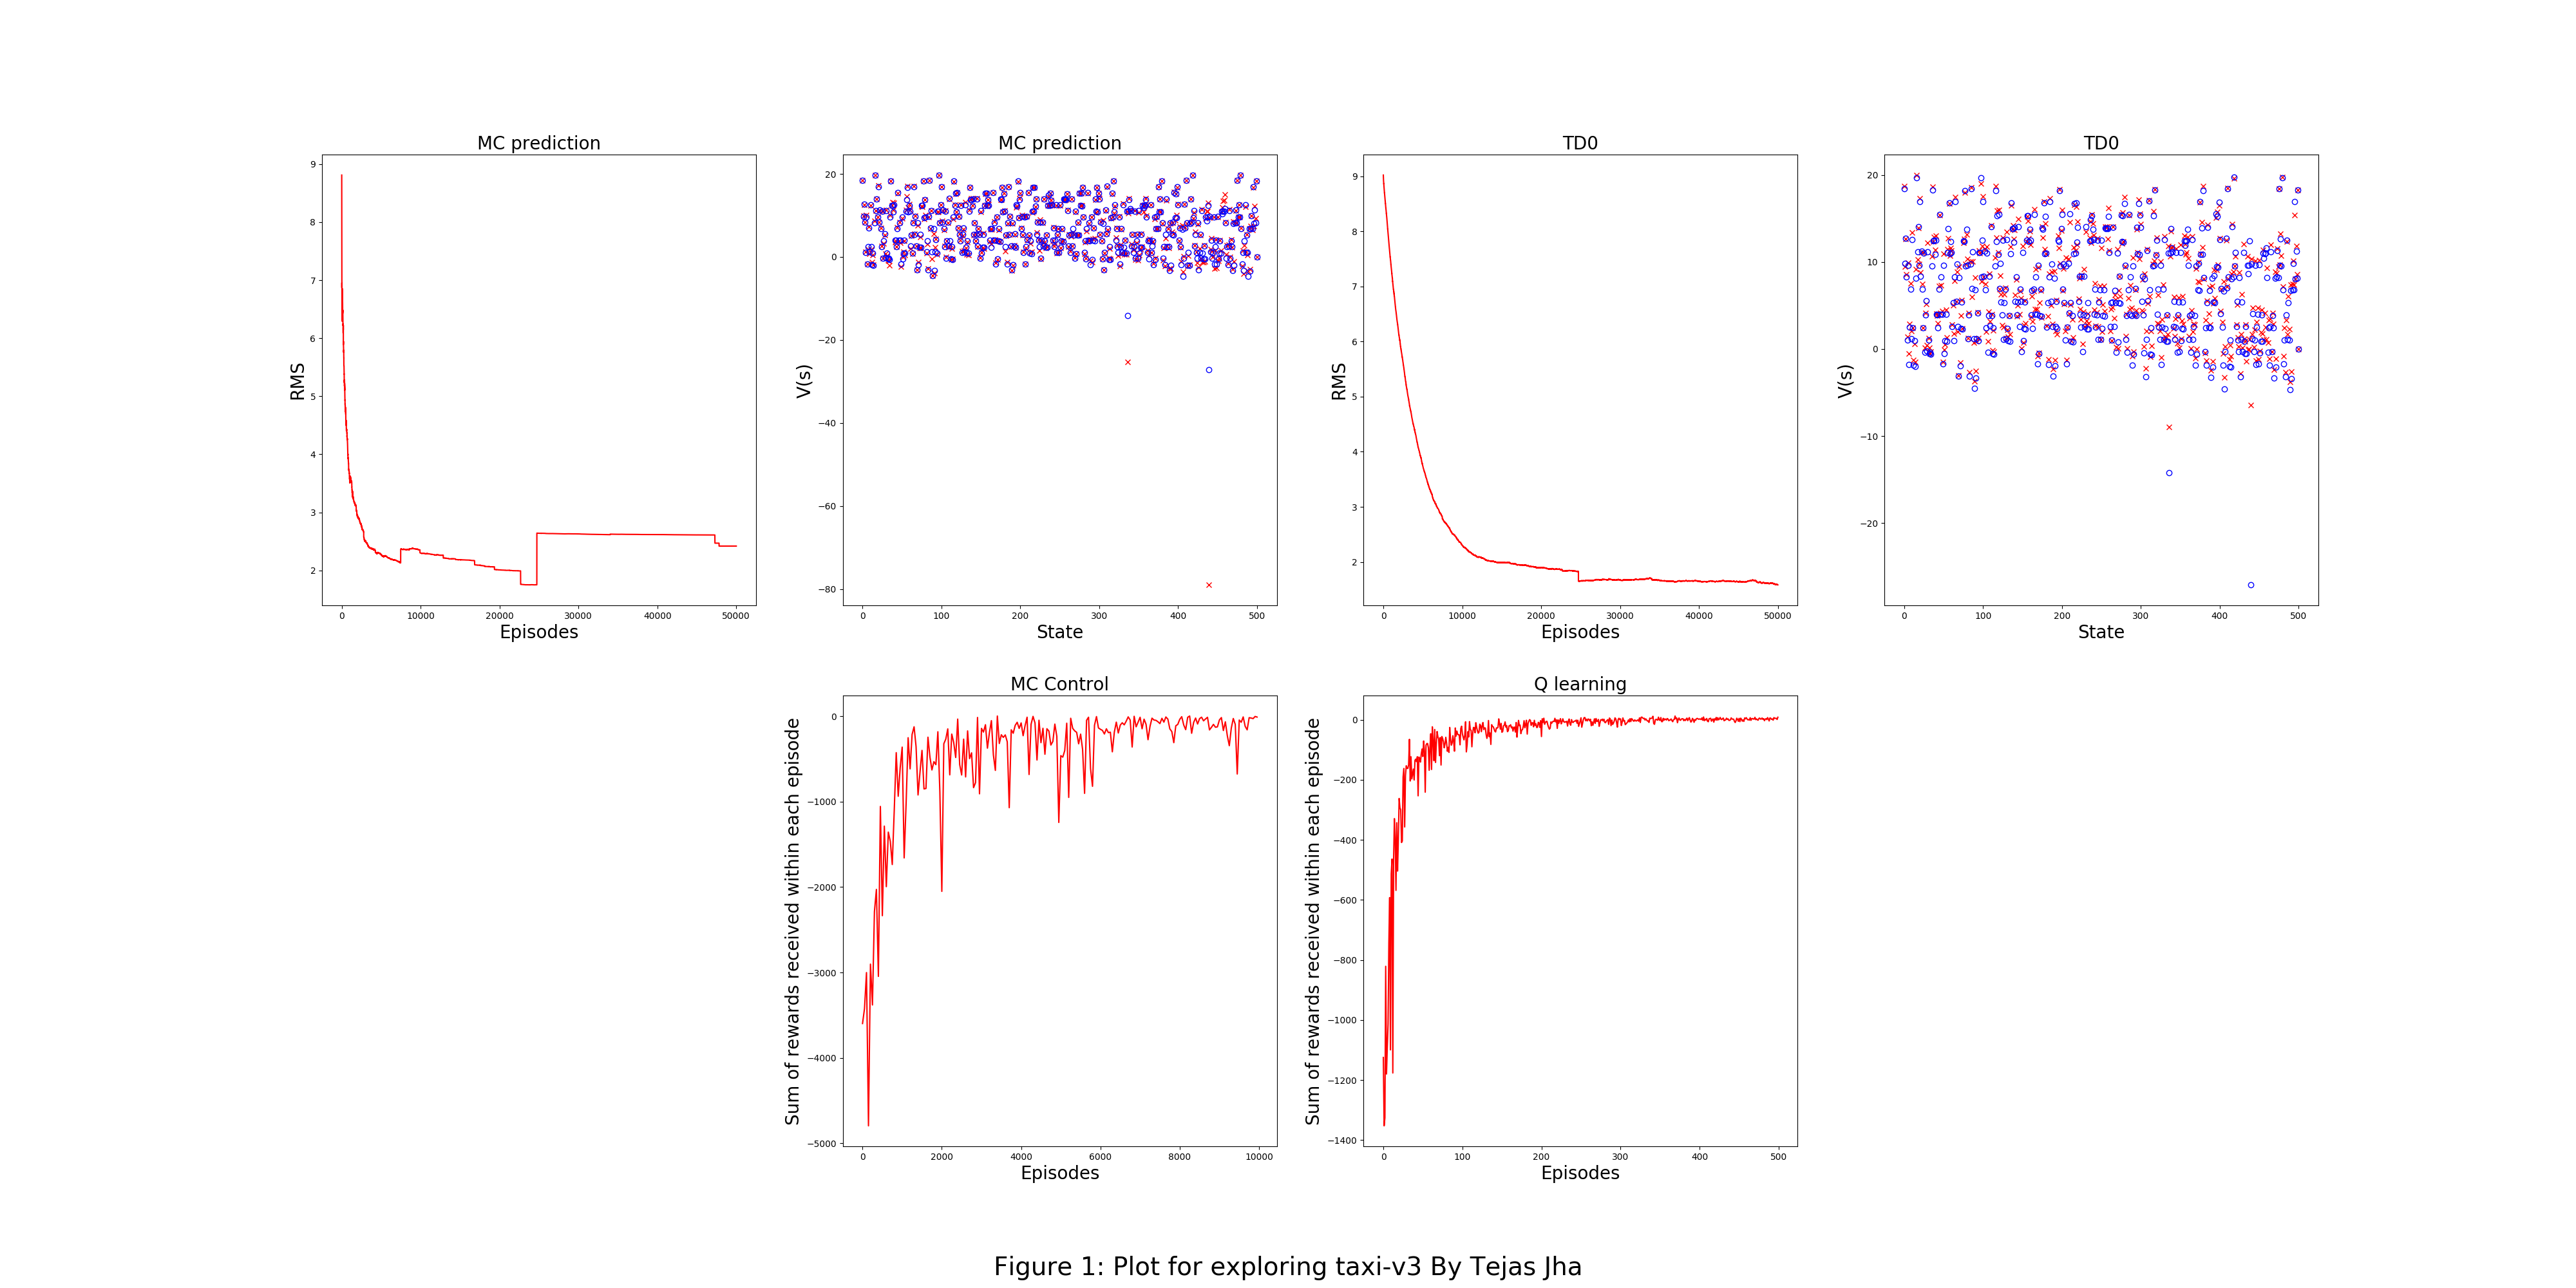
\includegraphics[scale = 0.4]{Figure3.png}

   \begin{figure}
       \noindent\makebox[\textwidth]{%
       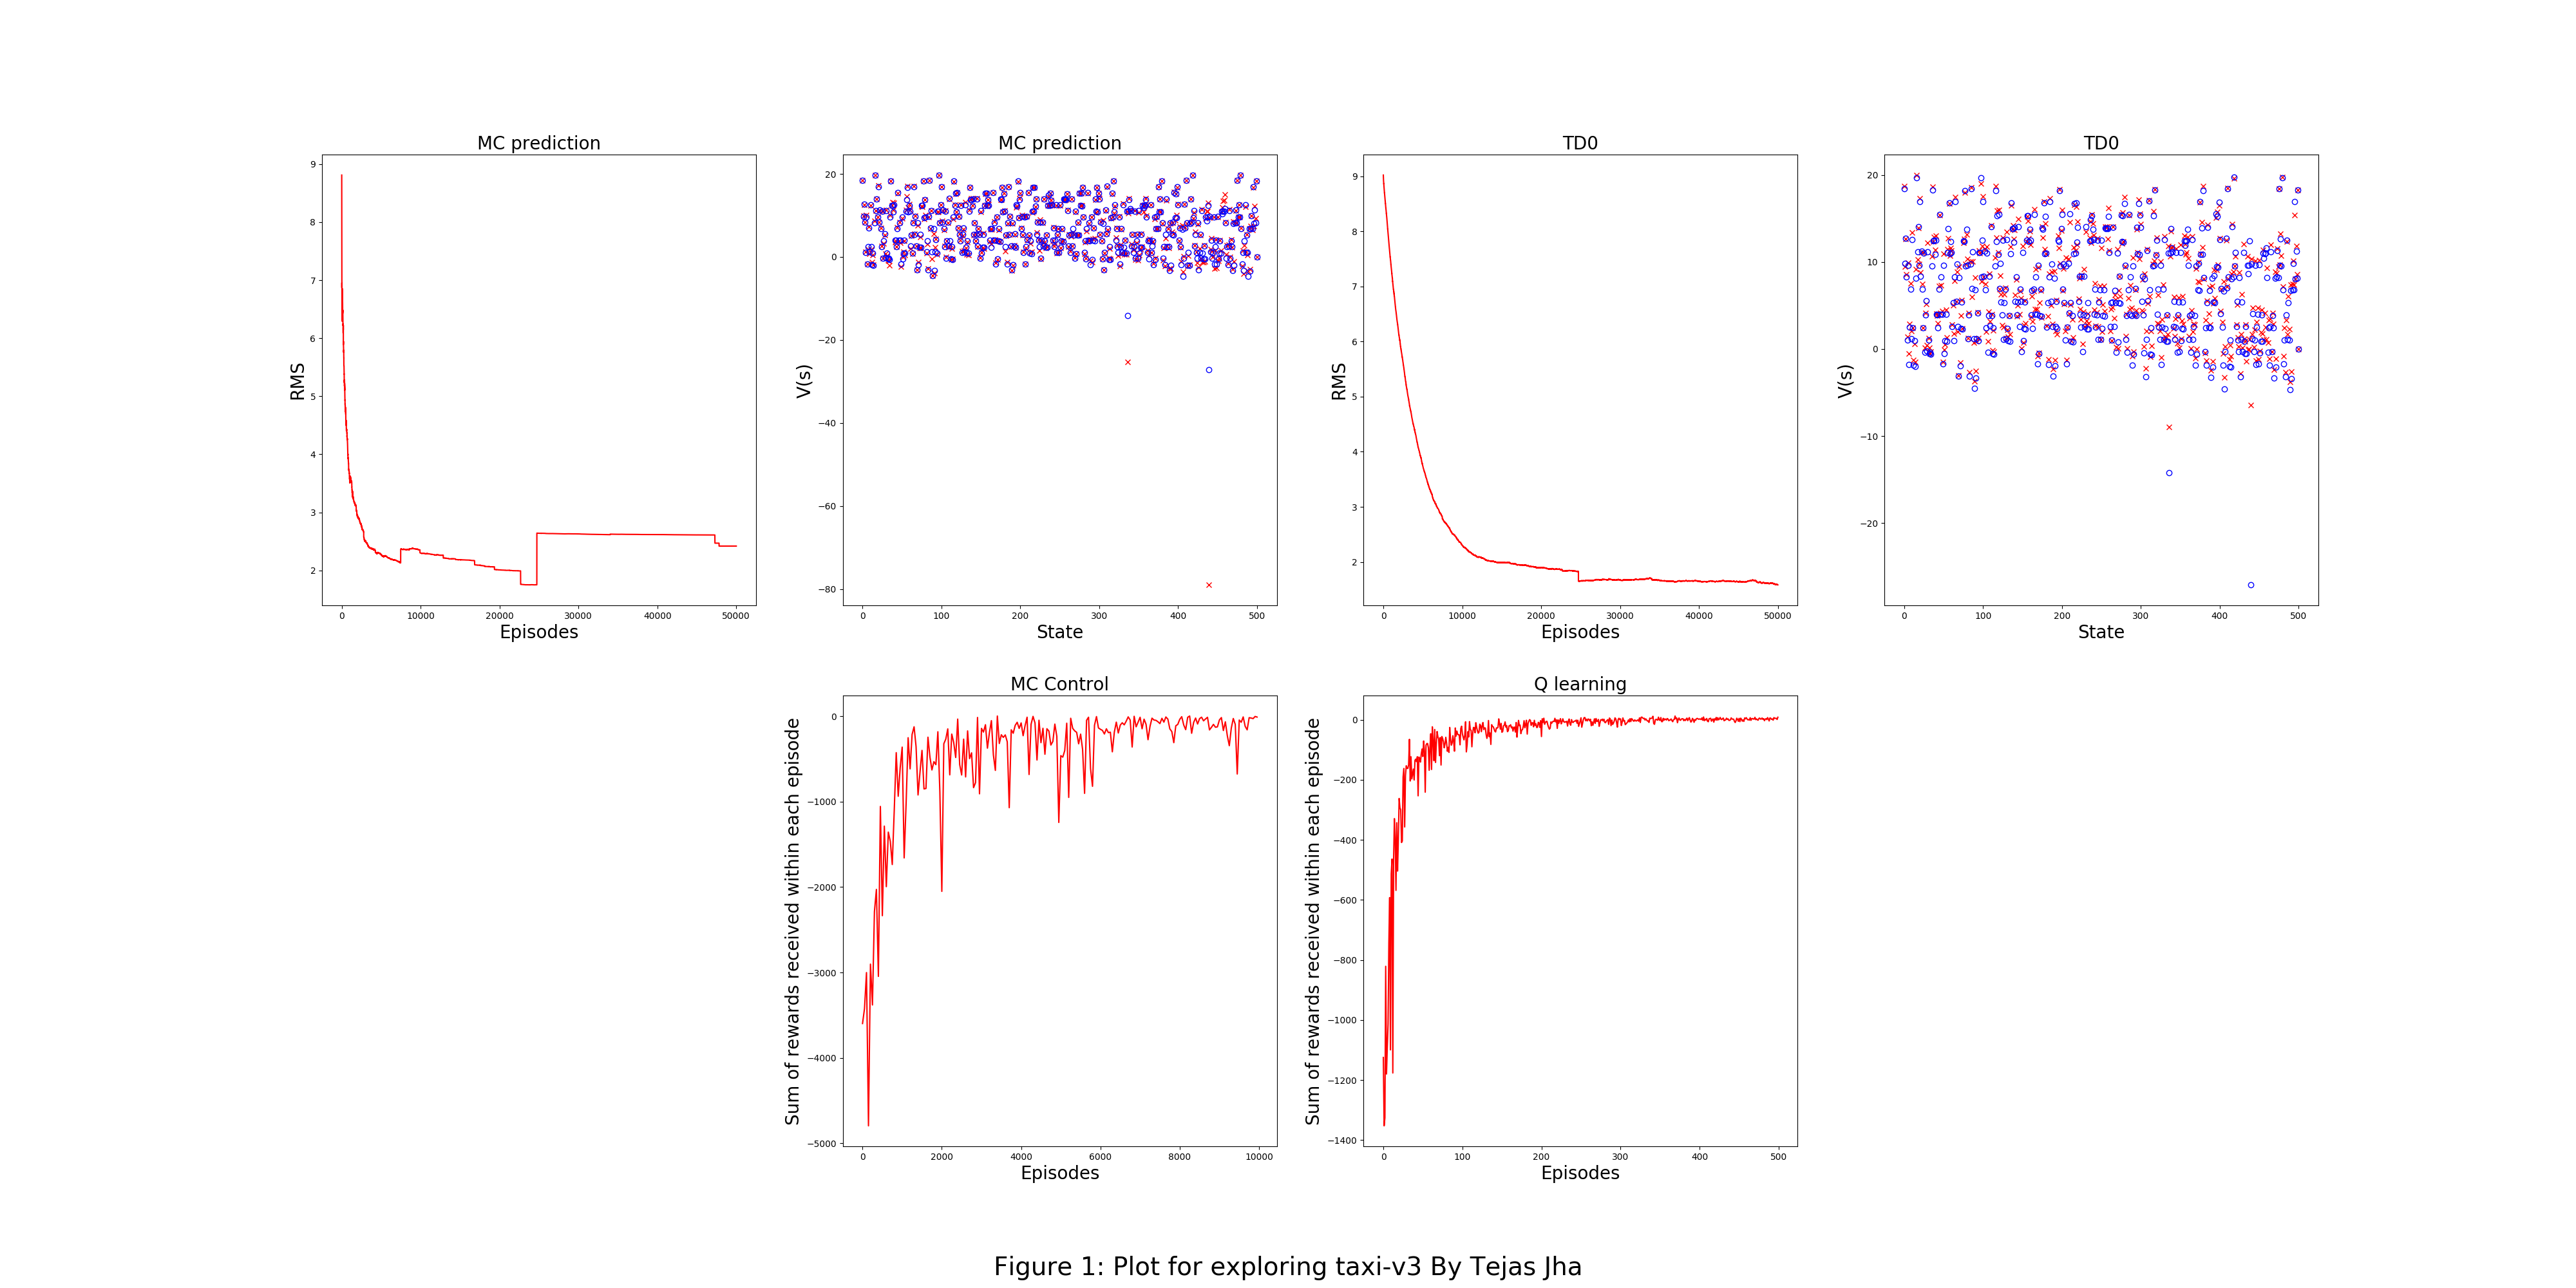
\includegraphics[width=1.6\textwidth]{Figure3.png}}
    \end{figure}


\clearpage

\section*{Appendix: Relevant Code - tjha.py}
\lstinputlisting[language=Python, breaklines=true, numbers=left]{tjha.py}   
\end{document}
